\documentclass[11pt, letterpaper]{memoir}
\usepackage{HomeworkStyle}
\geometry{margin=0.75in}



\begin{document}

	\begin{center}
		{\large Quiz 11.3 -- Vibrational Spectroscopy}
	\end{center}
	{\large Name: \rule[-1mm]{4in}{.1pt} 

\subsection*{Functional Groups}
These are infrared spectra for (in no particular order) a $\circ$ Nitrile, $\circ$ Alkane, $\circ$ Alcohol, and $\circ$ Ketone

\noindent
Label each spectra according to the correct functional group, and circle the feature or features on each infrared spectrum which you used to identify it

\noindent
\begin{tabular}{c|c}
	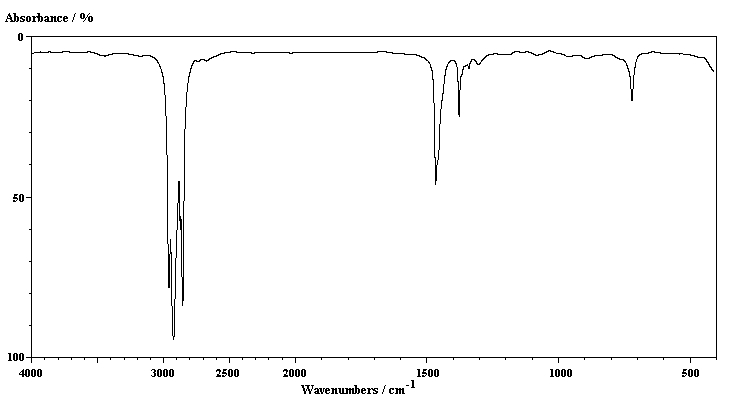
\includegraphics[width=0.49\linewidth]{Alkane} & 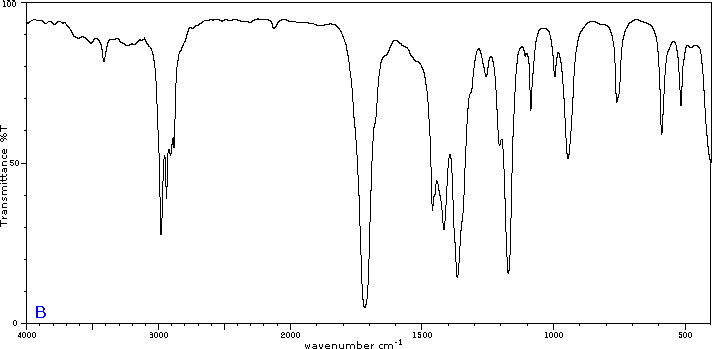
\includegraphics[width=0.49\linewidth]{Ketone} \\ \midrule
	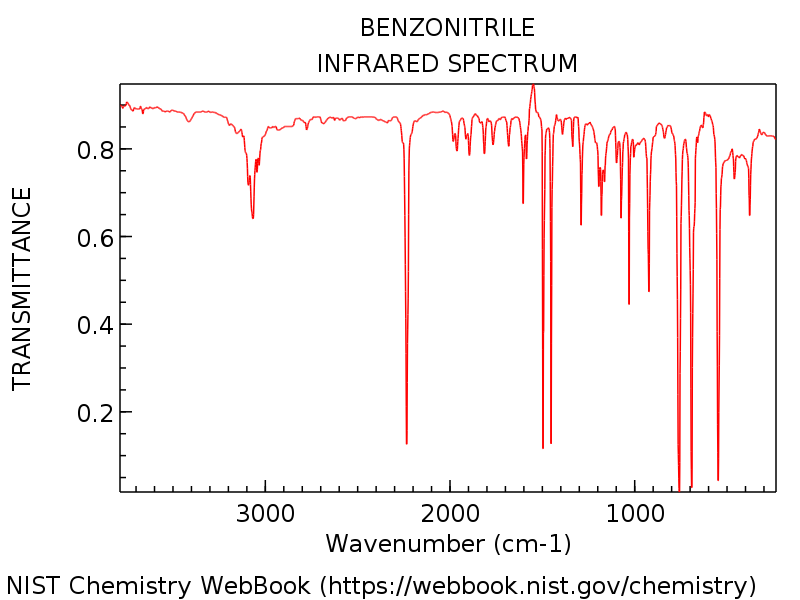
\includegraphics[width=0.49\linewidth, trim = 0 0 0 40, clip]{Nitrile} & 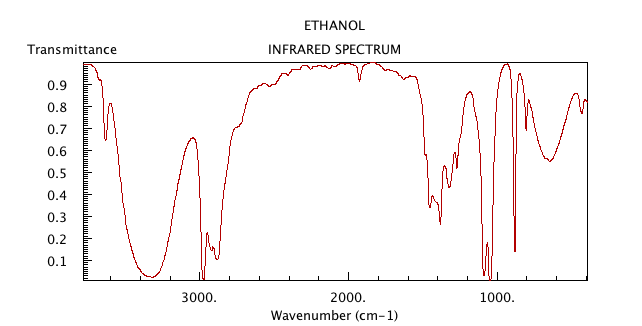
\includegraphics[width=0.49\linewidth, trim = 25 0 40 32, clip]{Alcohol}
\end{tabular}


\vspace{20em}
\subsection*{Ro-Vibrational Spectra}
	Below are IR and Raman spectra of the CN radical. Annotate them by labeling the following:
\begin{enumerate}
	\item O, P, Q, R, and S branches
	\item Initial and final states for the first 3 transitions in each branch
	\item $\alpha_e$	
	\item $\tilde{B}_e$, $\tilde{B}_0$, and $\tilde{B}_1$
\end{enumerate}

\noindent
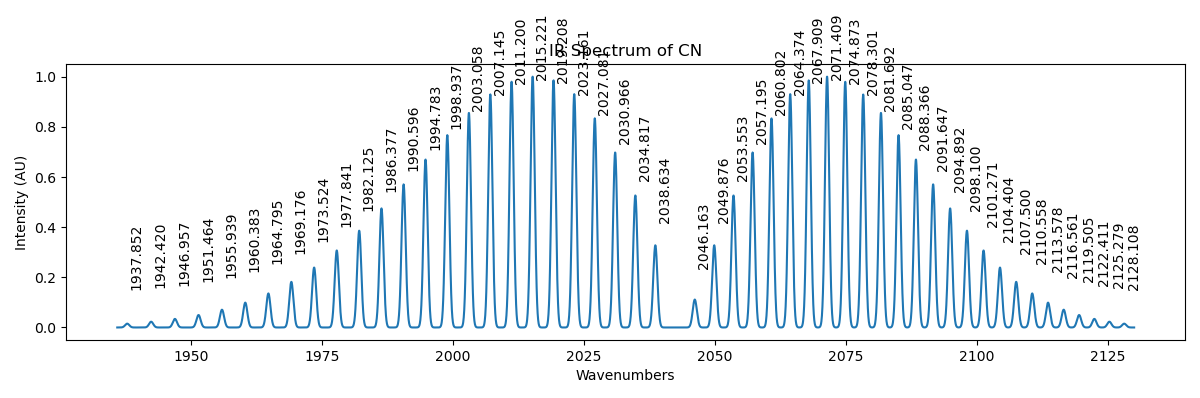
\includegraphics[trim= 0 0 0 0, clip=true, width=\linewidth]{CN_IR}

\noindent
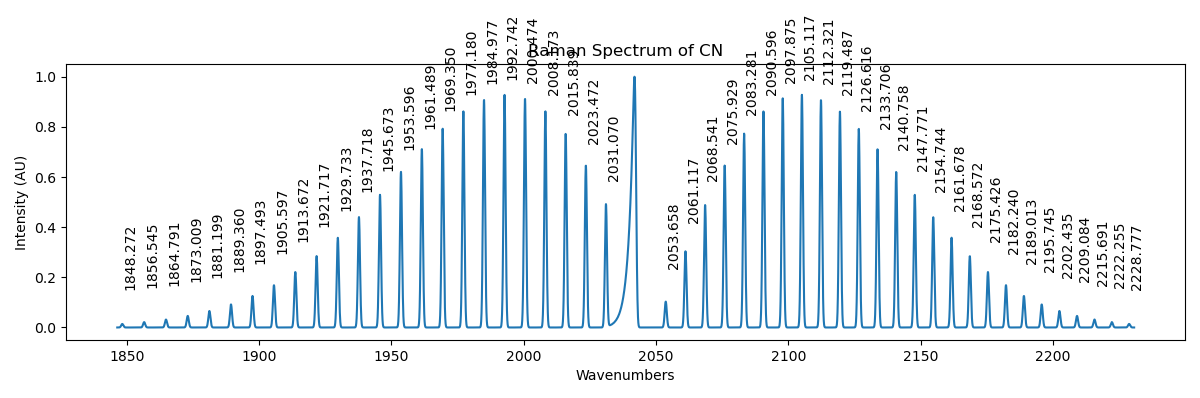
\includegraphics[trim= 0 0 0 0, clip=true, width=\linewidth]{CN_Raman}

\vspace{15em}
\subsection*{Vibrational Anharmonicity and Birge-Sponer Plots}
Below is a table of the first few vibrational transitions for the CN radical

\begin{tabular}{c|c}
	States & Energy ($cm^{-1}$) \\ \midrule
	$1\leftarrow0$ & $2042.416$ \\
	$2\leftarrow1$ & $2016.242$ \\
	$3\leftarrow2$ & $1990.068$ \\
	$4\leftarrow3$ & $1963.894$ \\
	$5\leftarrow4$ & $1937.720$ \\
\end{tabular}

\noindent
Draw or print a Birge-Sponer plot and give the following quantities:
\begin{enumerate}
	\item $\tilde{\nu}$
	\item $\chi_e\tilde{\nu}$
	\item $\tilde{D}_e$
	\item $\tilde{D}_0$
\end{enumerate}
\end{document}
